\section{NP-Completeness \S 34}

\begin{description}
	\item [P]  Class of problems {\it solvable} in polynomial time, {\it i.e.} $O(n^k)$ for some constant $k$.  
	\item [NP] Class of problems {\it verifiable} in polynomial time.  
	
	{\it Non-deterministic Polynomial time} or {\it Non-deterministic Polynomial acceptance problems}
	\item [NP-Complete] Class of problems in NP that is as hard as any other problem in NP.  
	\item [Optimization Problem] Given an undirected graph $G$ and vertices $u$ and $v$, find a path from $u$ to $v$ that uses the fewest edges.  
	\item [Decision Problem] Given an undirected graph $G$, vertices $u$ and $v$, and a constant $k$, is there a path from $u$ to $v$ consisting of at most $k$ edges?
	\item [Instance] An instance of a problem is a particular set of inputs to the problem.
\end{description}

	NP deals with decision problems, but the decision problem is no harder than the corresponding optimization problem.  If we show that the decision problem is NP-complete, then the optimization problem is NP-complete.  

\

\subsection{Polynomial-time Reduction Algorithm}

Given a decision problem $A$ we want to show can be solved in polynomial time, if we can show it is reducible in polynomial time to a decision problem $B$ known to be solvable in polynomial time, then we know $A$ can be solved in polynomial time.  

\begin{enumerate}
	\item Given an instance $\alpha$ of problem $A$, use a polynomial-time reduction algorithm to reduce it to an instance $\beta$ of problem $B$.  
	\item Run the polynomial-time decision algorithm for $B$ on the instance $\beta$.  
	\item Use the answer for $\beta$ as the answer for $\alpha$.  
\end{enumerate}

If the answer for each $\beta$ is the same as the answer for the corresponding $\alpha$, and if the transformation from $\alpha$ to $\beta$ takes polynomial time, and the solution for $\beta$ takes polynomial time, then we can use the transformation to $\beta$ to solve $\alpha$ in polynomial time.  


\subsection{Showing a Problem is NP-Complete}

We have a problem $B$ that we want to show is not in P.  

Assume that we have a decision problem $A$ for which we know that no polynomial-time algorithm can exist.  [Note that we are assuming that P is a proper subset of NP.]

Also assume that we have a polynomial-time transformation that maps instances of $A$ to instances of $B$.  

Prove by contradiction that $B \notin P$.  

Suppose $B$ has a polynomial-time algorithm.  Then, since we have a polynomial-time reduction transforming instances of $A$ to instances of $B$, there is a way to solve $A$ in polynomial time; however, this conclusion contradicts the given information that $A \notin P$.  Therefore, $B \notin P$.  

\subsection{Circuit Satisfiability \S 34.4}

To show that a problem, $B$, is NP-Complete, we first have to have a problem, $A$, known to be NP-Complete, so that we can find a polynomial-time reduction transforming instances of $A$ into instances of $B$.  

Our first NP-Complete problem will be the {\it Boolean satisfiability problem}, a.k.a. {\it propositional satisfiability}, {\it SAT}, {\it $k$-conjunctive normal form satisfiability}

A {\it truth assignment} for a boolean combinational circuit is a set of boolean input values.  A one-output boolean combinational circuit is {\it satisfiable} if it has a {\it satisfying assignment}, that is, a truth assignment that causes the output of the circuit to be 1.  The {\it circuit satisfiability problem} is, ``Given a boolean combinational circuit composed of AND, OR, and NOT gates, is it satisfiable?''  

In general, a {\it boolean combinational element} is a well-defined function that takes in a constant number of boolean inputs and returns a constant number of boolean outputs.  In this problem, the boolean combinational elements are the logic gates (AND, OR, NOT), each of which has a constant number of boolean inputs and one boolean output.  

A {\it boolean combinational circuit} has one or more boolean combinational elements (logic gates) connected by {\it wires}.  Each wire connects the output of one gate to the input of (at least one) other, making the output of the first gate an input for the second.  Wires can also take inputs from elsewhere and send outputs elsewhere.  

The {\it size} of a boolean combinational circuit is the number of boolean combinational elements (gates) plus the number of wires (including input/output from/to elsewhere).  If $k$ is the number of inputs in circuit $C$, then the size of the circuit is polynomial in $k$, and checking the problem has lower bound $\Omega(2^k)$ time.  The time is superpolynomial in the size of the circuit.  

\url{https://en.wikipedia.org/wiki/Boolean_satisfiability_problem}

\subsubsection{Example}

Figure 34.8, page 1072

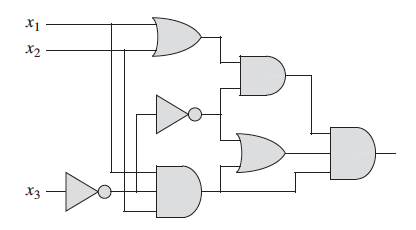
\includegraphics{Cormen_34_8.png}

I have labeled each of the logic gates, going left to right and top to bottom.  

\

\begin{tabular}{>{$}l<{$}}
	a = \lnot x_3 \cr
	b = x_1 \lor x_2 \cr
	c = \lnot a = x_3 \cr
	d = x_1 \land a \land x_2 = x_1 \land x_2 \land \lnot x_3 \cr
	e = b \land c = (x_1 \lor x_2) \land x_3 \cr
	f = c \lor d = x_3 \lor (x_1 \land x_2 \land \lnot x_3) = (x_1 \land x_2) \lor x_3 \cr
	g = e \land f \land d = ((x_1 \lor x_2) \land x_3) \land ((x_1 \land x_2) \lor x_3) \land (x_1 \land x_2 \land \lnot x_3) = (x_1 \land x_2) \land (x_3 \land \lnot x_3) \cr
\end{tabular}

\vskip 12pt

To test all of the inputs, we have $2^n$ inputs, where $n$ is the number of boolean variables.  Then we run each of those inputs through $k$ tests, where $k$ is the number of logic gates.  So we have $k\cdot 2^n$ tests, meaning that testing all of the inputs is $O(2^n)$.  

\

\begin{tabular}{*{12}{>{$}c<{$}|}}
	&&& a & b & c & d & e & f & g \cr
	x_1 & x_2 & x_3 & \lnot x_3 & x_1 \lor x_2 & \lnot a & x_1 \land a \land x_2 & b \land c & c \lor d & d \land e \land f \cr\hline
	0 & 0 & 0 & 1 & 0 & 0 & 0 & 0 & 0 & 0   \cr
	0 & 0 & 1 & 0 & 0 & 1 & 0 & 0 & 1 & 0   \cr
	0 & 1 & 0 & 1 & 1 & 0 & 0 & 0 & 0 & 0   \cr
	0 & 1 & 1 & 0 & 1 & 1 & 0 & 1 & 1 & 0   \cr
	1 & 0 & 0 & 1 & 1 & 0 & 0 & 0 & 0 & 0   \cr
	1 & 0 & 1 & 0 & 1 & 1 & 0 & 1 & 1 & 0   \cr
	1 & 1 & 0 & 1 & 1 & 0 & 1 & 0 & 1 & 0   \cr
	1 & 1 & 1 & 0 & 1 & 1 & 0 & 1 & 1 & 0  \cr
	
\end{tabular}

\

Direct method:  The problem is not satisfiable because we tested each of the instances and all of them failed.  

\

Heuristic (?) method:  The problem is not satisfiable because $d \land e = (x_1 \land x_2 \land \lnot x_3) \land ((x_1 \lor x_2) \land x_3) = x_1 \land (x_1 \lor x_2) \land x_2 \land x_3 \land \lnot x_3$, which depends on $x_3 \land \lnot x_3$ being true, which it is not for either value of $x_3$.  


\begin{lemma}
	The circuit-satisfiability problem belongs to NP.
\end{lemma}

\begin{proof}
	To ``belong to NP'' means to be verifiable in polynomial time.  We will give a sketch of a polynomial-time algorithm to verify an instance of the problem.  
	
	Two-input polynomial-time algorithm, $A$. 
	
	One input is a boolean combinational circuit, $C$  
	
	Second input is a {\it certificate} corresponding to an assignment of boolean values to the wires in the circuit $C$.
	
	  For each logic gate in $C$, the algorithm $A$ checks that the values of the output wire(s) are correctly computed from the values of the input wire(s).  If all of the computations are correct and the output of the entire circuit is 1, then the algorithm outputs 1.  Otherwise, (if any of the computations are incorrect, or if the output of the entire circuit is 0), then the algorithm $A$ returns 0.  
	  
	  For a satisfiable circuit $C$, there exists a certificate whose length is polynomial in the size of $C$ and that causes $A$ to output 1.   [Actually, the length of the certificate doesn't need to be larger than $C$.]  For an unsatisfiable circuit $C$, no certificate will return 1.  
	  
	  Since $A$ runs in (no worse than) polynomial time, we can verify the circuit satisfiability problem, so it belongs to NP.   
\end{proof}

\begin{lemma}
	The circuit-satisfiability problem is NP-hard.
\end{lemma}

\begin{proof}
	(To Do?)
\end{proof}

\begin{theorem}
	The circuit-satisfiability problem is NP-complete.
\end{theorem}

\begin{proof}
	Since the problem is both NP and NP-hard, by definition it is therefore NP-complete.
\end{proof}

\subsubsection{3-CNF or 3-P SAT}

A {\it literal} is an occurrence of a variable or its negation.  A boolean formula is in {\it conjunctive normal form} if it is expressed as an AND of clauses, each of which is an OR of one or more literals.  A boolean formula is in {\it 3-conjunctive normal form} or {\it 3-CNF} if each clause has exactly three distinct literals.  

The 3-CNF-SAT problem asks whether a given boolean formula $\phi$ in 3-CNF is satisfiable.  

\begin{theorem}
	Satisfiability of boolean formulas in 3-conjunctive normal form is NP-complete.  
\end{theorem}

Sketch of proof.  Need to prove that 3-CNF-SAT $\in$ NP and 3-CNF-SAT $\in$ NP-hard.   

To show that 3-CNF-SAT $\in$ NP, we show that there is a polynomial-time algorithm, $A$, to verify an instance of the problem.  The algorithm $A$ has two inputs, the boolean combinational circuit $C$ and a certificate corresponding to an assignment of boolean values to the wires in $C$.  To verify, we need to check that, for each gate, the boolean values on the input wires give the result on the output wire, and that the value of the final output wire is 1.  This verification algorithm is $O(|C|)$, where $|C|$ is the number of wires plus the number of gates; therefore, we have a polynomial-time algorithm that verifies any instance of the problem; therefore, 3-CNF-SAT $\in$ NP.  

To show that 3-CNF-SAT $\in$ NP-hard, we will show that SAT $\le_p$ 3-CNF-SAT, where ``$\le_p$'' is the {\it polynomial-time reducibility relation}. We do that by showing that every boolean combinational circuit satisfactiability problem can be transformed in polynomial time into a 3-conjunctive normal form satisfiability problem.  A general SAT problem cannot take longer than 3-CNF-SAT problems, because if it did, you could transform it into a 3-CNF-SAT problem and solve it; therefore, SAT $\le_p$ 3-CNF-SAT, and since SAT $\in$ NP-Complete, we have 3-CNF-SAT $\in$ NP-hard.  

Since 3-CNF-SAT $\in$ NP and 3-CNF-SAT $\in$ NP-hard, 3-CNF-SAT $\in$ NP-Complete.  {\it Q.E.D.}

\subsubsection{Example on page 1082 of reduction algorithm from SAT to 3-CNF-SAT}

\begin{align*}
\phi &= ((x_1 \to x_2) \lor \lnot (( \lnot x_1 \leftrightarrow x_3) \lor x_4)) \land \lnot x_2\cr
\phi &= 
\underbrace{
	\underbrace{
		((  
			\underbrace{x_1 \to x_2}_{y_3 = x_1 \to x_2}
		) \lor
		\underbrace{\lnot (  
			\underbrace{( 
				\underbrace{\lnot x_1 \leftrightarrow x_3}_{y_6 = \lnot x_1 \leftrightarrow x_3}
				) \lor x_4}_{y_5 = y_6 \lor x_4}
			)}_{y_4 = \lnot y_5}
	}_{y_2 = y_3 \lor y_4}
		) \land \lnot x_2
}_{y_1 = y_2 \land \lnot x_2}
	\cr
\end{align*}

\

Binary Parse Tree

\

\begin{tikzpicture}[x=6mm, y=10mm]
	\node (A) at (0,0) {$\phi$};
	\node [circle, draw, label=above right:$y_1$] (B) at (0,-1) {$\land$};
	\node [circle, draw, label=above right:$y_2$] (C) at (-8,-2) {$\lor$};
	\node [] (D) at (8,-2) {$\lnot x_2$};
	\node [circle, draw, label=above right:$y_3$] (E) at (-12,-3) {$\to$};
	\node [circle, draw, label=above right:$y_4$] (F) at (-4,-3) {$\lnot$};
	\node [] (G) at (-14,-4) {$x_1$};
	\node [] (H) at (-10,-4) {$x_2$};
	\node [circle, draw, label=above right:$y_5$] (I) at (-4,-4) {$\lor$};
	\node [circle, draw, label=above left:$y_6$] (J) at (-6,-5) {$\leftrightarrow$};
	\node [] (K) at (-2,-5) {$x_4$};
	\node [] (L) at (-7,-6) {$\lnot x_1$};
	\node [] (M) at (-5,-6) {$x_3$};
	
	\foreach \from/\to in {A/B, B/C, B/D, C/E, C/F, E/G, E/H, F/I, I/J, I/K, J/L, J/M}
		\draw (\from) -- (\to);
\end{tikzpicture}

\

\begin{tabular}{ *{10}{ >{$}c<{$}| } }
	&&&& y_3 & y_6 & y_5 & y_4 & y_2 & y_1 \cr
	x_1 & x_2 & x_3 & x_4 
		& x_1 \to x_2 
		& \lnot x_1 \leftrightarrow x_3 
		& y_6 \lor x_4 
		& \lnot y_5
		& y_3 \lor y_4 
		& y_2 \land \lnot x_2
	\cr\hline 
	0 & 0 & 0 & 0 & 1 & 0 & 0 & 1 & 1 & 1 \cr
	0 & 0 & 0 & 1 & 1 & 0 & 1 & 0 & 1 & 1 \cr  
	0 & 0 & 1 & 0 & 1 & 1 & 1 & 0 & 1 & 1 \cr  
	0 & 0 & 1 & 1 & 1 & 1 & 1 & 0 & 1 & 1 \cr  
	0 & 1 & 0 & 0 & 1 & 0 & 0 & 1 & 1 & 0 \cr  
	0 & 1 & 0 & 1 & 1 & 0 & 1 & 0 & 1 & 0 \cr  
	0 & 1 & 1 & 0 & 1 & 1 & 1 & 0 & 1 & 0 \cr  
	0 & 1 & 1 & 1 & 1 & 1 & 1 & 0 & 1 & 0 \cr  
	1 & 0 & 0 & 0 & 0 & 1 & 1 & 0 & 0 & 0 \cr  
	1 & 0 & 0 & 1 & 0 & 1 & 1 & 0 & 0 & 0 \cr  
	1 & 0 & 1 & 0 & 0 & 0 & 0 & 1 & 1 & 1 \cr  
	1 & 0 & 1 & 1 & 0 & 0 & 1 & 0 & 0 & 0 \cr  
	1 & 1 & 0 & 0 & 1 & 1 & 1 & 0 & 1 & 0 \cr  
	1 & 1 & 0 & 1 & 1 & 1 & 1 & 0 & 1 & 0 \cr  
	1 & 1 & 1 & 0 & 1 & 0 & 0 & 1 & 1 & 0 \cr  
	1 & 1 & 1 & 1 & 1 & 0 & 1 & 0 & 1 & 0 \cr  
\end{tabular}

\

See \verb|Reduction_1082.py|

\

We can rewrite a logical function $f$ on $a$ and $b$, $f(a,b)$, by introducing a variable $y$ that has the same value as $f(a,b)$, {\it i.e.} $y$ is true when $f(a,b)$ is true and $y$ is false when $f(a,b)$ is false.  They have the same value when $y \leftrightarrow f(a,b)$ is true.  We know that $f(a,b)$ is true when $y \land (y \leftrightarrow f(a,b))$ is true.  We can chain these together to get a formula $\phi'$ equivalent to $\phi$, as a conjunction of clauses $\phi'_i$ with at most three literals.  

\begin{align*}
	\phi' = y_1 &\land (y_1 \leftrightarrow (y_2 \land \lnot x_2)) \cr
		& \land (y_2 \leftrightarrow( y_3 \lor y_4 )) \cr
		& \land (y_3 \leftrightarrow( x_1 \to x_2 )) \cr
		& \land (y_4 \leftrightarrow( \lnot y_5 )) \cr
		& \land (y_5 \leftrightarrow( y_6 \lor x_4 )) \cr
		& \land (y_6 \leftrightarrow( \lnot x_1 \leftrightarrow x_3 )) \cr
\end{align*}

Below are the rows of the truth table for which $\phi' = 1$.  Note that they are the same values for $x_i$ as in $\phi$.  

\

\begin{tabular}{ *{12}{ |>{$}c<{$} } }
x_1 & x_2 & x_3 & x_4 & y_1 & y_2 & y_3 & y_4 & y_5 & y_6 & \phi' \cr\hline
0 & 0 & 0 & 0 & 1 & 1 & 1 & 1 & 0 & 0 & 1 &  \cr
0 & 0 & 0 & 1 & 1 & 1 & 1 & 0 & 1 & 0 & 1 &  \cr
0 & 0 & 1 & 0 & 1 & 1 & 1 & 0 & 1 & 1 & 1 &  \cr
0 & 0 & 1 & 1 & 1 & 1 & 1 & 0 & 1 & 1 & 1 &  \cr
1 & 0 & 1 & 0 & 1 & 1 & 0 & 1 & 0 & 0 & 1 &  \cr\end{tabular}

\

Now we have a formula $\phi'$ that is a conjunction of clauses $\phi'_i$, each of which has at least three literals.  To be in 3-conjunctive normal form, we need it to be a conjunction of clauses, each of which is a disjunction of exactly three literals.  To go from $\phi'$ to $\phi''$, follow these steps.  

\begin{enumerate}
	\item Make a truth table for each clause $\phi_i'$.  
	\item Using each entry that evaluates to 0, build a formula in disjunctive normal for (an OR of ANDs) that is equivalent to $\lnot \phi_i'$.
	\item Negate this formula and convert it into a CNF formula $\phi_i''$ using DeMorgan's laws for propositional logic, particularly that $\lnot (a \land b) = \lnot a \land \lnot b$ to complement all literals, changing ORs to ANDs and vice versa.  Now we have converted each clause $\phi_i'$ into a conjunctive normal form $\phi_i''$ with at most three literals.  
	\item If a clause $\phi_i''$ has fewer than three literals, pad it.  
	\item Take the conjunction of all of the clauses.  
\end{enumerate}

\begin{tabular}{*9{|>{$}c<{$}}}
	x_2 & y_1 & y_2 & y_2 \land \lnot x_2 & y_1 \leftrightarrow (y_2 \land \lnot x_2) & \text{DNF for } \lnot \phi_2' &  \text{CNF for } \phi_2'' \cr\hline
	1  & 1 & 1 & 0 & 0 & x_2 \land y_1 \land y_2 & \lnot x_2 \lor \lnot y_1 \lor \lnot y_2 \cr
	1  & 1 & 0 & 0 & 0 & x_2 \land y_1 \land \lnot y_2  & \lnot x_2 \lor \lnot y_1 \lor y_2  \cr
	1  & 0 & 1 & 0 & 1 && \cr
	1  & 0 & 0 & 0 & 1 && \cr
	0  & 1 & 1 & 1 & 1 && \cr
	0  & 1 & 0 & 0 & 0 & \lnot x_2 \land y_1 \land \lnot y_2  & x_2 \lor \lnot y_1 \lor  y_2  \cr
	0  & 0 & 1 & 1 & 0 & \lnot x_2 \land \lnot y_1 \land y_2  & x_2 \lor y_1 \lor \lnot y_2  \cr
	0  & 0 & 0 & 0 & 1 && \cr
\end{tabular}

$$\text{CNF:} \qquad \phi_2'' =  (\lnot x_2 \lor \lnot y_1 \lor \lnot y_2) \land ( \lnot x_2 \lor \lnot y_1 \lor y_2  ) \land (x_2 \lor \lnot y_1 \lor  y_2 ) \land ( x_2 \lor y_1 \lor \lnot y_2  )$$

\begin{tabular}{*9{|>{$}c<{$}}}
	x_2 & y_1 & y_2 & 
	\lnot x_2 \lor \lnot y_1 \lor \lnot y_2 &
	\lnot x_2 \lor \lnot y_1 \lor y_2 &
	x_2 \lor \lnot y_1 \lor  y_2 &
	x_2 \lor y_1 \lor \lnot y_2 & \phi_2'' \cr\hline
	1 & 1 & 1 & 0 & 1 & 1 & 1 & 0 \cr
	1 & 1 & 0 & 1 & 0 & 1 & 1 & 0 \cr
	1 & 0 & 1 & 1 & 1 & 1 & 1 & 1 \cr
	1 & 0 & 0 & 1 & 1 & 1 & 1 & 1 \cr
	0 & 1 & 1 & 1 & 1 & 1 & 1 & 1 \cr
	0 & 1 & 0 & 1 & 1 & 0 & 1 & 0 \cr
	0 & 0 & 1 & 1 & 1 & 1 & 0 & 0 \cr
	0 & 0 & 0 & 1 & 1 & 1 & 1 & 1 \cr
\end{tabular}

\

$\phi_5'$ has only two literals.  

\

\begin{tabular}{*9{|>{$}c<{$}}}
	y_4 & y_5 & y_4 \leftrightarrow \lnot y_5 & \lnot \phi_5' & \phi_5'' & \text{CNF for } \phi_5'' \cr\hline
	1 & 1 & 1 &  &  & \cr
	1 & 0 & 0 &  y_4 \land \lnot y_5 & \lnot y_4 \lor y_5 & (\lnot y_4 \lor y_5 \lor p) \land (\lnot y_4 \lor y_5 \lor \lnot p) \cr
	0 & 1 & 0 &  \lnot y_4 \land y_5 &y_4 \lor \lnot y_5  & (y_4 \lor \lnot y_5 \lor p) \land (y_4 \lor \lnot y_5 \lor \lnot p) \cr
	0 & 0 & 1 &  &  & \cr
\end{tabular}

$$\phi_5'' =  (\lnot y_4 \lor y_5 \lor p) \land (\lnot y_4 \lor y_5 \lor \lnot p) \land  (y_4 \lor \lnot y_5 \lor p) \land (y_4 \lor \lnot y_5 \lor \lnot p)  $$

\

$\phi_1'$ has only one literal.  

\

\begin{tabular}{*9{|>{$}c<{$}}}
	y_1 & \lnot \phi_1' & \phi_1'' & {\text CNF for } \phi_1'' \cr\hline
	1 &  && \cr
	0 & \lnot y_1 & y_1 & (y_1 \lor p \lor q) \land (y_1 \lor p \lor \lnot q) \land (y_1 \lor \lnot p \lor q) \land (y_1 \lor \lnot p \lor \lnot q)  \cr
\end{tabular}

\

This $p,q$ thing might make more sense if we put it in the table.  

\

\begin{tabular}{*9{|>{$}c<{$}}}
 	y_1 & p & q & y_1 & \lnot \phi_1' & \text{CNF for } \phi_1'' \cr\hline
 	1 & 1 & 1 & 1 &  &  \cr
 	1 & 1 & 0 & 1 &  &  \cr
 	1 & 0 & 1 & 1 &  &  \cr
 	1 & 0 & 0 & 1 &  &  \cr
 	0 & 1 & 1 & 0 & \lnot y_1 \land p \land q & y_1 \lor \lnot p \lor \lnot q \cr
 	0 & 1 & 0 & 0 & \lnot y_1 \land p \land \lnot q & y_1 \lor \lnot p \lor q  \cr
 	0 & 0 & 1 & 0 & \lnot y_1 \land \lnot p \land q  & y_1 \lor p \lor \lnot q  \cr
 	0 & 0 & 0 & 0 & \lnot y_1 \land \lnot p \land \lnot q  & y_1 \lor p \lor q  \cr
\end{tabular}

\

This conversion to 3-CNF takes polynomial time, so we have a polynomial-time reduction from SAT to 3-CNF-SAT; therefore, 3-CNF-SAT is at least as hard as SAT.  Since SAT is NP-complete and SAT $\le_p$ 3-CNF-SAT, we have 3-CNF-SAT is NP-complete.  

\subsubsection{2-CNF-SAT}

A 2-CNF is boolean formula in conjunctive normal form with exactly two literals per clause, like $(a \lor b) \land (\lnot a \lor b) \land (a \lor c)$.  

The interesting thing about 2-CNF is that $a \lor b \equiv \lnot a \to b \equiv \lnot b \to a$.  Use the pairs of implications to make an implication graph, a directed graph that is skew symmetric (if you swap the negations

A 2-CNF formula is satisfiable if and only if there is no variable that belongs to the same strongly connected component as its negation.  

To show that a boolean expression in 2-conjunctive normal form is satisfiable, 

\begin{enumerate}
	\item Write as an implication graph. 
	\item Use DFS or Kosaraju's algorithm to find the strongly connected components.  
	\item Check whether any strongly-connected component contains both a variable and its negation.  
\end{enumerate}

Each of these steps can be done in polynomial time, so the whole process can be done in polynomial time, so 2-CNF-SAT $\in$ P.

%%%%%
\subsection{Traveling Salesman Problem}

\subsubsection{TSP as a decision problem}

\begin{tabular}{lll}
	TSP = &$\{ (G, c, k)$: 
		& $G = (V,E)$ is a complete graph. \cr
		&& $c$ is a cost function from $V \times V \to \mathbb{N}$ \cr
		&& $k \in \mathbb{N}$, and \cr
		&& $G$ has a traveling-salesman tour with cost at most $k$. \cr
		&\} \cr
\end{tabular}

\

The traveling-salesman tour is a Hamiltonian cycle, visiting each node exactly once and returning to the starting point.  

To show that TSP $\in$ NP-complete, (a) show that TSP $\in$ P by walking through what it would take to confirm a solution and saying that it can be done in polynomial time, and (b) show that HAM-CYCLE $\le_P$ TSP by saying that HAM-CYCLE is a special case of TSP.  Since HAM-CYCLE is NP-complete, TSP is also.  

Let $G = (V,E)$ be an instance of HAM-CYCLE.  Form a complete graph $G' = (V, E')$ where $E' = \{(i,j): i,j \in V \text{ and } i \ne j\}$.  Define the cost function by $c(i,j) = 0 \text{ if } (i,j) \in E, 0 \text{ if } (i,j) \notin E$.  The instance of TSP is $(G', c, 0)$.  

The graph $G$ is a hamiltonian cycle iff graph $G'$ has a tour of cost at most 0.  

\subsubsection{Triangle Inequality}

If the cost function has the property that cutting out an intermediate stop never increases the cost, {\it i.e.} the most direct path between two points is not more expensive than a meandering one, {\it i.e.} the triangle inequality holds on the cost function, $c(u,w) \le c(u,v) + c(v,w)$, the problem is still NP-complete, but we can use Prim's algorithm for a minimal spanning tree to find, in polynomial time, an approximate solution whose total cost is no more than twice the optimal solution.  

%%%
\subsubsection{	S19 \#S6}
Many problem have been proved to be NP-complete.  To prove NP-completeness, it is necessary in general to demonstrate two proof components.  What are the two proof components to show a problem being NP-complete?
	
	Being NP-complete, the traveling-salesman problem (TSP) has a 2-approximation solution in polynomial time based on establishing a minimum spanning tree (MST) rooted at the start/end vertex (in polynomial time following MST-PRIM), if the graph edge weights observe the triangle inequality.  Sketch a brief proof to demonstrate that that such a proof satisfies 2-approximation.  



%%%%%
\subsection{Knapsack Problem}

%%%
\subsubsection{	S18 \#L4}
\begin{enumerate}[label=\alph*.]
		\item Define the following classes of a decision problem:  P, NP, and NP-completeness.
		\item Consider the 0-1 knapsack problem with $n$ objects each with its respective pre-defined profit.  The objective is to maximize the total profit that can be accommodated into a container of capacity $W$.  Define appropriate notations for weight and profit of objects, formulate the problem.
		\item Convert of the problem that you have defined in (b) into a decision problem.
		\item Show the problem that you have defined in (c) belongs to NP-class.
		\item Does the problem in (d) belong to the P-class or NP-completeness. (Justify your answer.)
		\item If principle of optimality be applicable to solve the problem defined in (c), formulate it.  Otherwise, explain why not.  
		\item What would be your explanation, if 0-1 knapsack problem is solved by dynamic programming in polynomial time?
\end{enumerate}

%%%%%
\subsection{Old Exam Problems}

%%%
\subsubsection{S15 \#L1}

\begin{enumerate}
		\item Suppose you have to find a solution to a problem that belongs to NP-complete class.  Clearly summarize the steps that will help you to find the solution of the problem.  
		\item John, an undergraduate student, recently took data structure course, states that heuristics algorithms always solve NP-complete problems.  He cites simplex methods as an example.  If you agree with John, justify why or why not.  
		\item What is the strategy behind a greedy algorithm?  Will it always provide an optimal solution?  If yes explain why, otherwise say why not.  
		\item Consider the following pseudo code for Kruskal's algorithm for solving minimal spanning tree (MST).

Algorithm MST.  Let $N$ be the number of nodes in graph $G$.  

\begin{lstlisting}[numbers=left, mathescape=True]
Sort the edges in non-decreasing order of cost.
$T$ is an empty graph
while $T$ has fewer than $N-1$ edges do:
	let $e$ denote the next edge of $G$ (in the order of cost)
	if $T \cup \{e\}$ does not contain a cycle, then $T = T \cup \{e\}$
\end{lstlisting}

Clearly mentioning the data structure you have to employ to reduce the time complexity to access and to maintain the necessary information, show the exact time taken to obtain the MST.  Also show the tight bound of the algorithm.  (Pay attention in detecting a cycle.)
\end{enumerate}

%%%
\subsubsection{Solutions}

1.  [From \S 35, page 1106]  There are three ways to approach an NP-Complete problem.  

a.  If the problem size is sufficiently small that, even if the growth is exponential or factorial, the time and resources required to solve it directly are within the time and money budgets, you may solve it directly.  

b.  See if the instances you are considering form a special case of the problem that can be solved in polynomial time.  

c.  Find an approximate solution.  

\

%%%
\subsubsection{S15 \#L3}

\begin{enumerate}
		\item Compare and contrast P, NP, NP-Complete, and NP-Hard.
		\item Based on current conjecture, draw a Venn diagram to show the relationship among these classes of problem.
		\item Clearly state what is understood by propositional satisfiability problem. 
		\item Suppose there are $m$ clauses and $k$ propositions in a given 3-p sat problem.  How many possible interpretations are there?  What is the time complexity of testing the satisfiability of a given interpretation?  What is the time and space complexity of testing the satisfiability of the clauses?
		\item Suppose you came across a research paper that highlights a clever heuristic strategy that the authors have used to solve an instance of 3-p sat which has 10,000 propositions and 10,000 clauses with 3 propositions.  They have generated several instances of the similar compositions of variables and clauses.  The authors, in their point of view, have demonstrated the power of their heuristic to solve an instance of NP-complete problem in polynomial time (empirically shown).  What would be your insight of their findings?
\end{enumerate}

\subsubsection{Solutions}

\begin{enumerate}
	\item 
	
\begin{description}
	\item [P] Solvable in polynomial time
	\item [NP] Verifiable in polynomial time
	\item [NP-Complete] Verifiable in polynomial time and at least as hard to solve as any other problem in NP
	\item [NP-Hard] At least as hard to solve as any other problem in NP, but not necessarily verifiable in polynomial time.  
\end{description}	

	$\text{P} \subset \text{NP}$
	
	$\text{NP-Complete} \subset \text{NP}$

	$\text{NP-Complete} \subset \text{NP-Hard}$
	
	$\text{NP-Complete} = \text{NP} \cap \text{NP-Hard}$
	
	The open question is whether there are problems verifiable in polynomial time that are not solvable in polynomial time.  

	\item \

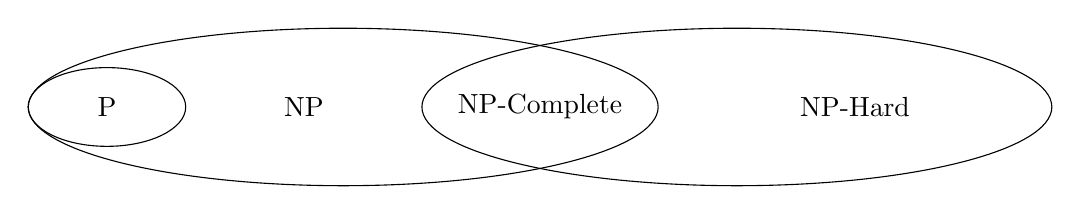
\begin{tikzpicture}[x=10mm, y=5mm]
	\draw (0,0) ellipse (4 and 2); 
	\node () at (-0.5,0) {NP};
	\draw (5,0) ellipse (4 and 2);
	\node () at (6.5,0) {NP-Hard};
	\draw (-3,0) circle (1) node {P};
	\node () at (2.5,0) {NP-Complete};
\end{tikzpicture}

	% #3
	\item A propositional satisfiability problem asks, given a boolean combinational circuit composed of some number of inputs, AND, OR, and NOT gates, and single output, is there a set of inputs that will yield a TRUE (1) output? 

\end{enumerate}

%%%
\subsubsection{F15 \#S5}
Mark True or False for each of the following statements.  
\begin{enumerate}[label=\alph*.]
		\item Greedy strategy sometimes finds the best or the optimal solution.
		\item Dynamic programming will always find the optimal solution even when the principal of optimality condition is not satisfied.
		\item (Same as S5 \#S9b) Breadth first search is a special case of heuristic search algorithm.
		\item Some problems that belong to NP-class can be solved polynomially.  
		\item Satisfiability problem of propositional calculus is NP-complete.
\end{enumerate}

\subsubsection{Solutions}

\begin{enumerate}[label=\alph*.]
	\item
	\item
	\item
	\item  True.  Being NP means they can be verified in polynomial time.  It does not mean they cannot be solved in polynomial time.  
	\item  True.  There are some special cases, like 2-CNF, but in general, SAT is NP-complete.
\end{enumerate}

%%%
\subsubsection{F16 \#S5}

Suppose there are $n$ clauses and $m$ variables (propositions) in a given $3-p$ sat problem.
\begin{itemize}
	\item How many possible interpretations are there?
	\item Find the tight bound of checking for satisfiability of the $n$ clauses.  
\end{itemize}

%%%
\subsubsection{F16 \#L1}

\begin{enumerate}
	\item Briefly describe NP-class, P-class, NP-complete, and NP-hard.
	\item Show the conjectured relationship among the classes NP-class, P-class, NP-complete, and NP-hard.
	\item Show that counting $n$ objects with integer key values belongs to NP-class.  
	\item Provide the steps involved in showing whether a problem belongs to NP-complete or not.
	\item Illustrate the steps in step d by showing 3 proposition satisfiability (3-p sat) problem belongs to NP-complete.
	\item Provide a pseudo code that attempt to solve 3-p sat problem heuristically.
\end{enumerate}

%%%
\subsubsection{S17 \#L2}
\begin{enumerate}[label=\alph*.]
		\item Compare and contrast P, NP, NP-complete, and NP-hard.
		\item Based on current conjecture, draw a Venn diagram to show the relationship among these classes of problem.
		\item Suppose there $n$ clauses and $m$ propositions in a given 3p-sat problem.  How many possible interpretations are there?  What is the time complexity of testing the satisfiability of a given interpretation?  What is the time and space complexity of testing the satisfiability of the clauses?
		\item 3-p sat problem is NP-complete, but people still have published papers by applying heuristics strategy and showing that they were able to solve it with large number of distinct propositions (say 100) and large number of clauses (say 200).  To avoid any bias, they have generated the clauses and the set of propositions randomly.  How would you start investigating their results?  Can their results be generalized?
		\item Suppose a single NP-complete problem is solved in polynomial algorithm, what can you state about the entire NP-complete class as well as the NP-hard class.
\end{enumerate}

\subsubsection{Solutions}

\begin{enumerate}[label=\alph*.]
	% a.
	\item
	\begin{description}
		\item [P]  Solvable in polynomial time.  $O(n^k)$ for constant $k$.  
		\item [NP] Verifiable in polynomial time.  May or may not be solvable in polynomial time.  
		\item [NP-complete] Verifiable in polynomial time, but at least as hard to solve as any problem in NP.  Conjectured to not have a polynomial-time solution.  
		\item [NP-hard]  Both verification and solution are as hard as for any problem in NP.   Not known to be verifiable or solvable in polynomial time.  Conjectured to have polynomial-time methods for neither verification nor solution.  
	\end{description}
	
	P $\subset$ NP
	
	NP-complete $\subset$ NP
	
	NP-complete = NP $\cap$ NP-hard
	
	% b.
	\item \
	
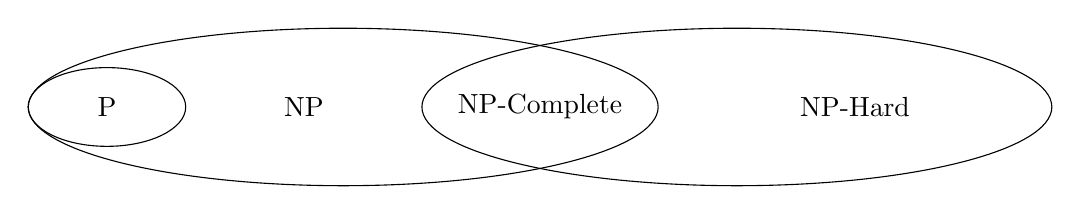
\begin{tikzpicture}[x=10mm, y=5mm]
	\draw (0,0) ellipse (4 and 2); 
	\node () at (-0.5,0) {NP};
	\draw (5,0) ellipse (4 and 2);
	\node () at (6.5,0) {NP-Hard};
	\draw (-3,0) circle (1) node {P};
	\node () at (2.5,0) {NP-Complete};
\end{tikzpicture}

	% c.
	\item  I assume by ``number of propositions'' they mean ``number of propositional variables'' or ``number of variables.''  I don't find this topic in the textbook.  
	
	The number of interpretations (instances?) is $2^m$.  
	
	The truth table has $2^m$ rows and $m+n+1$ columns.  The first $m$ columns are just loop assignment.  The next $n$ columns evaluate the 3-disjunction clauses, each of which should take constant time.  The last column evaluates the conjunction of the $n$ clauses for each instance, which should take time proportional to the number $n$ of clauses.  
		
	So setting up and evaluating each row (interpretation, instance) should take $O(m+n+n) = O(m+n)$.  Since $m/2 \le n$, we can write that as $O(n)$.  Since there are $2^m$ rows, our total time is $O(n \cdot 2^n)$.  The memory required for testing the satisfiability of a clause is also $O(n)$.  
	
	
	
	% d.
	\item
	
	% e.
	\item A problem is NP-complete if it is at least as difficult as every problem in NP, {\it i.e.} a problem $A$ is NP-complete if, for every problem $B \in$ NP, there is a polynomial-time transformation $f$ such that any instance $\beta \in B$ can be transformed into an instance of $A$, so that $f(\beta) = \alpha \in A$.  The problem $A$ is at least as hard as $B$ because, if it were easier, we could use the solution method for $A$ to solve $B$.  
	
	 If a single NP-complete problem, like $A$, is solved in polynomial time, then each problem $B \in $ NP could be solved in polynomial time by transforming (in polynomial time) each instance of $B$ into an instance of $A$.  Thus, if one NP-complete problem could be solved in polynomial time, each and every NP problem (including each NP-complete problems) could be solved in polynomial time.  
	 
	 Finding a polynomial-time solution to an NP-complete problem would have no similar effect on the NP-hard problems that are not NP.  The definition of NP-hard says that each of those problems is at least as hard as each of the NP problems, but does not specify that it is at least as hard as any other NP-hard problems.  Taking down one does not make the group fall.  
	
\end{enumerate}

%%%
\subsubsection{	S18 \#L4}
\begin{enumerate}[label=\alph*.]
		\item Define the following classes of a decision problem:  P, NP, and NP-completeness.
		\item Consider the 0-1 knapsack problem with $n$ objects each with its respective pre-defined profit.  The objective is to maximize the total profit that can be accommodated into a container of capacity $W$.  Define appropriate notations for weight and profit of objects, formulate the problem.
		\item Convert of the problem that you have defined in (b) into a decision problem.
		\item Show the problem that you have defined in (c) belongs to NP-class.
		\item Does the problem in (d) belong to the P-class or NP-completeness. (Justify your answer.)
		\item If principle of optimality be applicable to solve the problem defined in (c), formulate it.  Otherwise, explain why not.  
		\item What would be your explanation, if 0-1 knapsack problem is solved by dynamic programming in polynomial time?
\end{enumerate}

\subsubsection{Solutions}

\begin{enumerate}[label=\alph*.]
	\item 
	\begin{description}
		\item [P] Solvable in polynomial time
		\item [NP] Verifiable in polynomial time
		\item [NP-complete] Verifiable in polynomial time, but at least as hard to solve as any other problem in NP.  Conjectured to not have a solution in polynomial time.  
	\end{description}
	
	P $\subset$ NP, NP-complete $\subset$ NP.
	
\end{enumerate}

%%%
\subsubsection{	S19 \#S6}
Many problem have been proved to be NP-complete.  To prove NP-completeness, it is necessary in general to demonstrate two proof components.  What are the two proof components to show a problem being NP-complete?
	
	Being NP-complete, the traveling-salesman problem (TSP) has a 2-approximation solution in polynomial time based on establishing a minimum spanning tree (MST) rooted at the start/end vertex (in polynomial time following MST-PRIM), if the graph edge weights observe the triangle inequality.  Sketch a brief proof to demonstrate that that such a proof satisfies 2-approximation.  

\subsubsection{Solution}

\begin{description}
	\item [First Part]
	
	NP-complete problems are the intersection of two sets, NP problems and NP hard problems.  To prove that a problem is NP-complete, we show that it belongs to both sets.  
	
	To prove that a problem is NP-complete, there are two steps.  First, we show that it is NP, meaning that a solution can be verified in polynomial time.  Second, we show that it is NP-hard, meaning that it is at least as hard to solve as a known (or conjectured) NP-hard problem.  
	
	\item [Second Part]
\end{description}

